\documentclass{subfiles}

\begin{document}

    \chapter{Implementaciones sobre el sistema de Realidad Aumentada}
    \label{chap:3}

        \section{Modelo en 3D y Three.js}
        \label{sec:3.1}
        A partir del sistema básico generado en el capítulo anterior, podemos empezar a añadirle complejidad a nuestro sistema. El primer elemento que añadiremos es un modelo en 3D que utilizaremos como base en esta aplicación.

        \paragraph{}
        Para la carga, inserción, control y movimientos de los modelos en 3D se ha utilizado en esta aplicación la librería \threejs. \threejs es una librería ligera preparada para su uso en aplicaciones web compatible con \js \cite{web:wikipediathreejs}. Además, este está especializado en el control de modelos en 3D en formato \glb y \gltf, que son dos formatos basados en \textit{JSON} y que están creados para ser óptimos en tiempo de ejecución (el formato \glb es el equivalente en binario a \gltf) \cite{web:threejs_loading3dmodels}.

        \paragraph{}
        La librería \threejs basa su funcionalidad en el uso de Escenas o \textit{Scenes}, el objeto que utiliza esta librería para acoger sus modelos en 3D, la iluminación o focos de luz que los alumbrarán y las cámaras virtuales que observarán a estos mismos \cite{web:threejs_scene}. Este último concepto es muy importante, debido a que afectará continuamente al renderizado de los modelos en 3D.

        \paragraph{}
        La cámara virtual es la que simula el punto de vista del espectador tanto en \ra como en \rv como en otras virtualizaciones que utilicen modelos en 3D como en simulaciones, videojuegos o películas de animación. A alto nivel, una cámara virtual, además de la posición del espectador, define también lo que este va a ver de manera que, cuando se va a renderizar una imagen, solo tiene que generarse la parte visible de los modelos que entren en el rango de visión de la cámara virtual.

        \begin{figure}
        \centering
        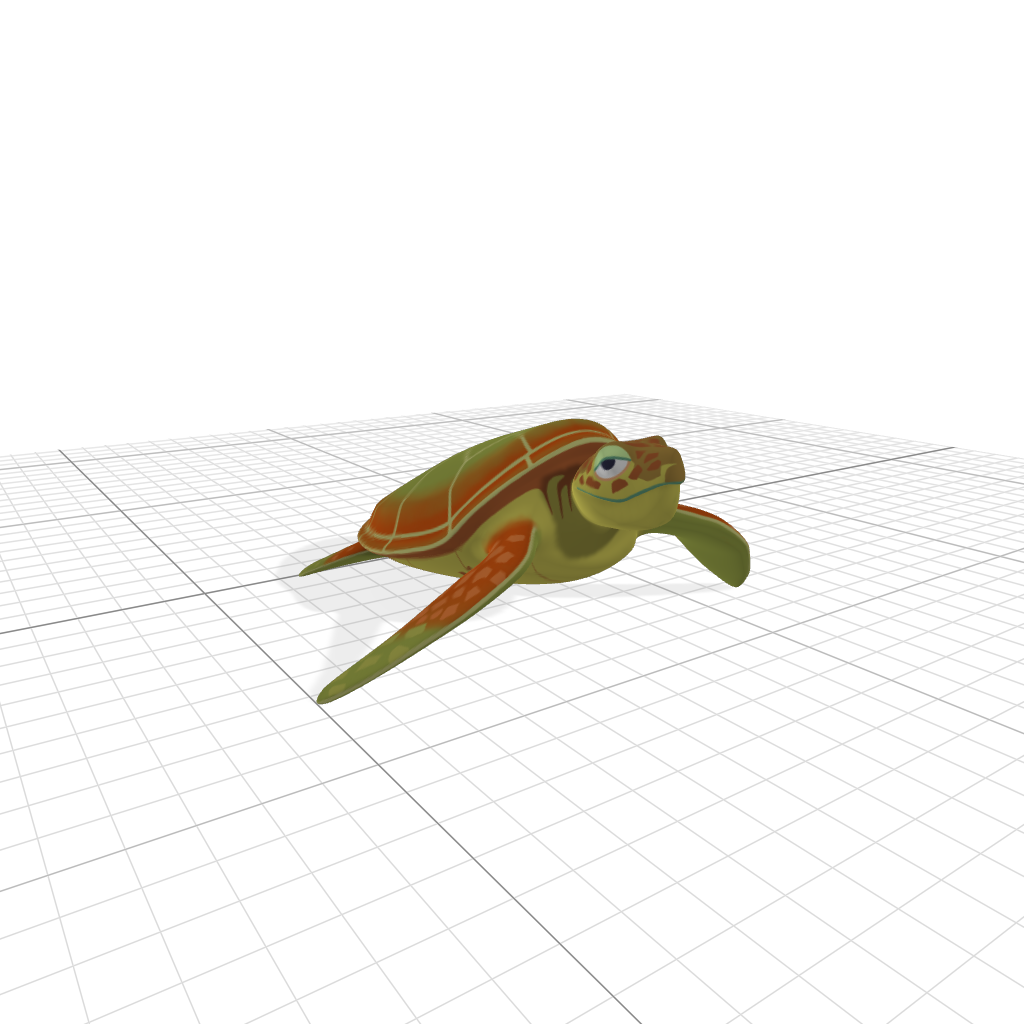
\includegraphics[width=0.6\textwidth]{img/tortuga_marina.png}
        \caption{Ejemplo de renderizado de un modelo en 3D extraído de la biblioteca de modelos 3D de la aplicación de Windows \textit{Visor 3D}.}
        \label{fig:tortuga_marina}
        \end{figure}

        \paragraph{}
        Visualizando esto último con un ejemplo, en la figura \ref{fig:tortuga_marina} se ha renderizado un modelo 3D de una tortuga marina. En este renderizado, la cámara virtual se encuentra frente al modelo, pero ligeramente ladeado hacia el lado derecho de la tortuga. Debido a la posición de la cámara, no es necesario que se renderice la pata izquierda trasera de la figura, puesto que lo tapa el resto del cuerpo. Sin embargo, si la cámara se encontrase detrás de la tortuga, sería necesario renderizar ambas patas traseras y la cola, pero no se renderizaría la cara de la figura.
        
        \paragraph{}
        Aunque este parezca un concepto obvio, es necesario explicarlo, debido a que será necesario establecer la posición y orientación de la cámara virtual durante el desarrollo. Esto es porque la cámara virtual coincidirá con la posición de la cámara del dispositivo móvil. Cuando la cámara apunte hacia una figura en 3D en la \ra, se incrustará en la pantalla del móvil la parte de la figura que se vea desde la cámara virtual (es decir, se debe ver por la pantalla lo que se vería a través de la cámara si esta figura existiese en nuestra Realidad).

        %% carga de figuras
        %% ubicacion de las figuras
        %% carga aleatoria de figuras

        \section{Cálculo de superficies, Hit Test Results}
        \label{sec:3.x}

        \section{Animación de modelos}
        \label{sec:3.y}
        %% clock
        %% comentar también el evento onTouch

        \section{Sonido espacial}
        \label{sec:3.z}
        %% comentar tambien el evento onsessionend

        \section{Funcionamiento final de la Realidad Aumentada}
        \label{sec:3.a}
        %% 

        

\end{document}